\documentclass{beamer}

\usetheme{default}
\usecolortheme{crane}

%%% Работа с русским языком
\usepackage{cmap}					% поиск в PDF
\usepackage{mathtext} 				% русские буквы в формулах
\usepackage[T2A]{fontenc}			% кодировка
\usepackage[utf8]{inputenc}			% кодировка исходного текста
\usepackage[english,russian]{babel}	% локализация и переносы
\usepackage{indentfirst}
\frenchspacing


%%% Дополнительная работа с математикой
\usepackage{amsmath,amsfonts,amssymb,amsthm,mathtools} % AMS
\usepackage{icomma} % "Умная" запятая: $0,2$ --- число, $0, 2$ --- перечисление

%% Номера формул
%\mathtoolsset{showonlyrefs=true} % Показывать номера только у тех формул, на которые есть \eqref{} в тексте.
%\usepackage{leqno} % Нумерация формул слева

%% Свои команды
\DeclareMathOperator{\sgn}{\mathop{sgn}}

%% Перенос знаков в формулах (по Львовскому)
\newcommand*{\hm}[1]{#1\nobreak\discretionary{}
	{\hbox{$\mathsurround=0pt #1$}}{}}

%%% Работа с картинками
\usepackage{graphicx}  % Для вставки рисунков
\graphicspath{{images/}}  % папки с картинками
\setlength\fboxsep{3pt} % Отступ рамки \fbox{} от рисунка
\setlength\fboxrule{1pt} % Толщина линий рамки \fbox{}
\usepackage{wrapfig} % Обтекание рисунков текстом
\usepackage{subfigure}

%%% Работа с таблицами
\usepackage{array,tabularx,tabulary,booktabs} % Дополнительная работа с таблицами
\usepackage{longtable}  % Длинные таблицы
\usepackage{multirow} % Слияние строк в таблице

%%% Программирование
\usepackage{etoolbox} % логические операторы

%
%\usepackage{fancyhdr} % Колонтитулы
% 	\pagestyle{fancy}
%\renewcommand{\headrulewidth}{0pt}  % Толщина линейки, отчеркивающей верхний колонтитул
% 	\lfoot{Нижний левый}
% 	\rfoot{Нижний правый}
% 	\rhead{Верхний правый}
% 	\chead{Верхний в центре}
% 	\lhead{Верхний левый}
%	\cfoot{Нижний в центре} % По умолчанию здесь номер страницы

\usepackage{setspace} % Интерлиньяж
%\onehalfspacing % Интерлиньяж 1.5
%\doublespacing % Интерлиньяж 2
%\singlespacing % Интерлиньяж 1

\usepackage{lastpage} % Узнать, сколько всего страниц в документе.

\usepackage{soul} % Модификаторы начертания


\usepackage{csquotes} % Еще инструменты для ссылок

%\usepackage[style=authoryear,maxcitenames=2,backend=biber,sorting=nty]{biblatex}

\usepackage{multicol} % Несколько колонок

\usepackage{tikz} % Работа с графикой
\usepackage{pgfplots}
\usepackage{pgfplotstable}

\renewcommand{\phi}{\varphi}
\renewcommand{\epsilon}{\varepsilon}
\usepackage[backend=biber]{biblatex}
\usepackage{usebib}
\usepackage[justification=centering, font=footnotesize]{caption}
\setbeamertemplate{caption}[numbered]

\addbibresource{./Semkin_2023_Lockdown.bib}
\bibinput{./Semkin_2023_Lockdown}

\author{Сёмкин Кирилл \\ Консультант: Антон Бишук}
\date{}
\title{Исследование распространения эпидемий в графовой модели SIR и влияния локдауна на динамику заболеваемости популяции}

\newcommand{\prob}{\ensuremath{\mathbb{P}}}
\newcommand{\matwait}{\ensuremath{\mathbb{E}}}

\begin{document}
	
	\begin{frame}[c]
		\titlepage
	\end{frame}

	\begin{frame}{Цели}
		
		\begin{itemize}
			\item Построить математическую модель распространения эпидемии типа SIR на графе
			\item Исследовать динамику заболеваемости при введении локдауна и без него
			\item Проиллюстрировать полученные теоретические/эмпирические оценки на численных экспериментах
		\end{itemize}
	
	\end{frame}

	\begin{frame}{Литература}
		
	{\large \textit{Основная работа}} \medskip
	
	\citeauthor{base_article}, ``\textit{\usebibentry{base_article}{title}}'' \bigskip
	
	{\large \textit{Связанные работы с моделированием эпидемии в среднем (mean field)}} \medskip
	
	\citeauthor{moreno2002epidemic}, ``\textit{\usebibentry{moreno2002epidemic}{title}}''
	
	\citeauthor{gomez2010discrete}, ``\textit{\usebibentry{gomez2010discrete}{title}}''
	
	\citeauthor{pastor2015epidemic}, ``\textit{\usebibentry{pastor2015epidemic}{title}}''
		
	\end{frame}

	\begin{frame}{Постановка задачи}
		
		Граф контактов $G(V,E)$. 
		
		Каждая вершина может быть в одном из трёх состояний:\textit{ Susceptable (S), Infected (I), Recovered (R)} --- по сути раскраска графа.
		
		\begin{center}
			\begin{figure}
				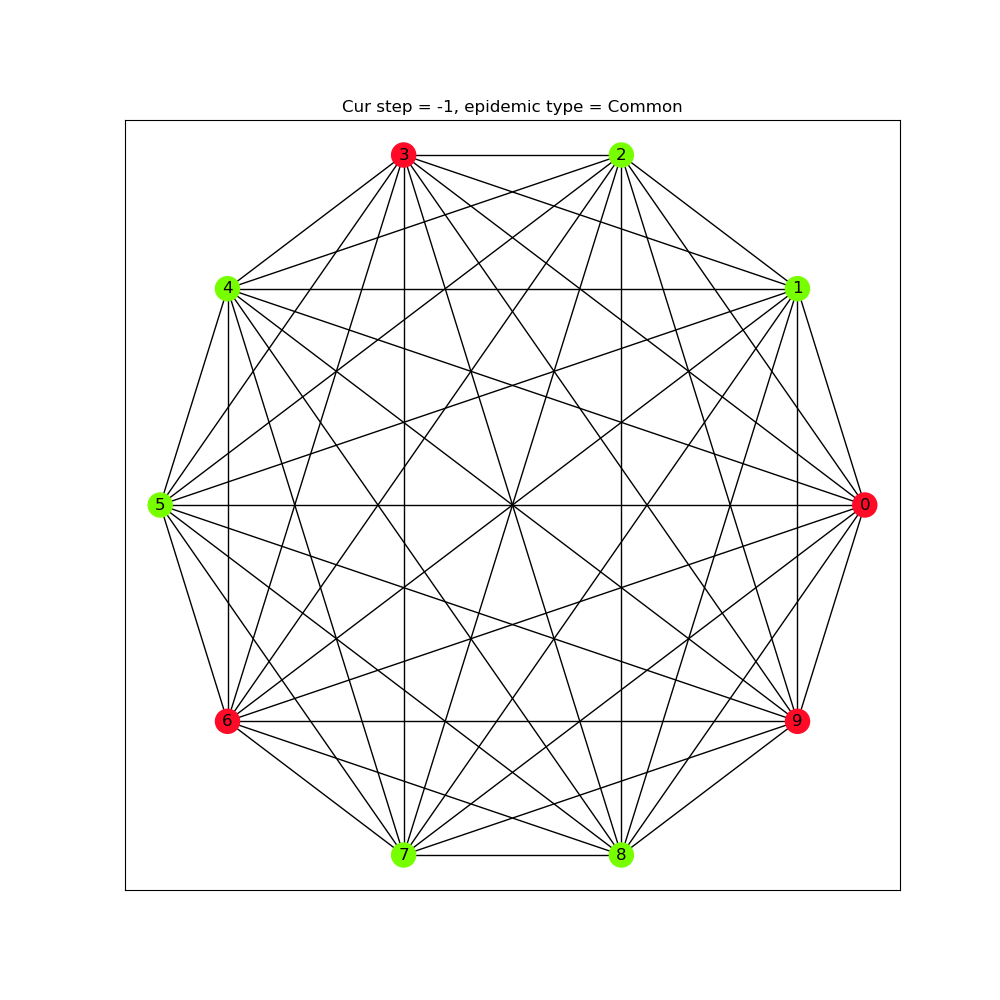
\includegraphics[width=0.5\linewidth]{../../figs/anti_evdence_1/init_config}
				\caption{Пример графа контактов с некоторым начальным распределением для вершин}
			\end{figure}
		\end{center}
		 
	\end{frame}

	\begin{frame}{Постановка задачи}
		
			\begin{figure}[t]
				\caption{Эволюция графа контактов во времени}
				\subfigure[Начало]{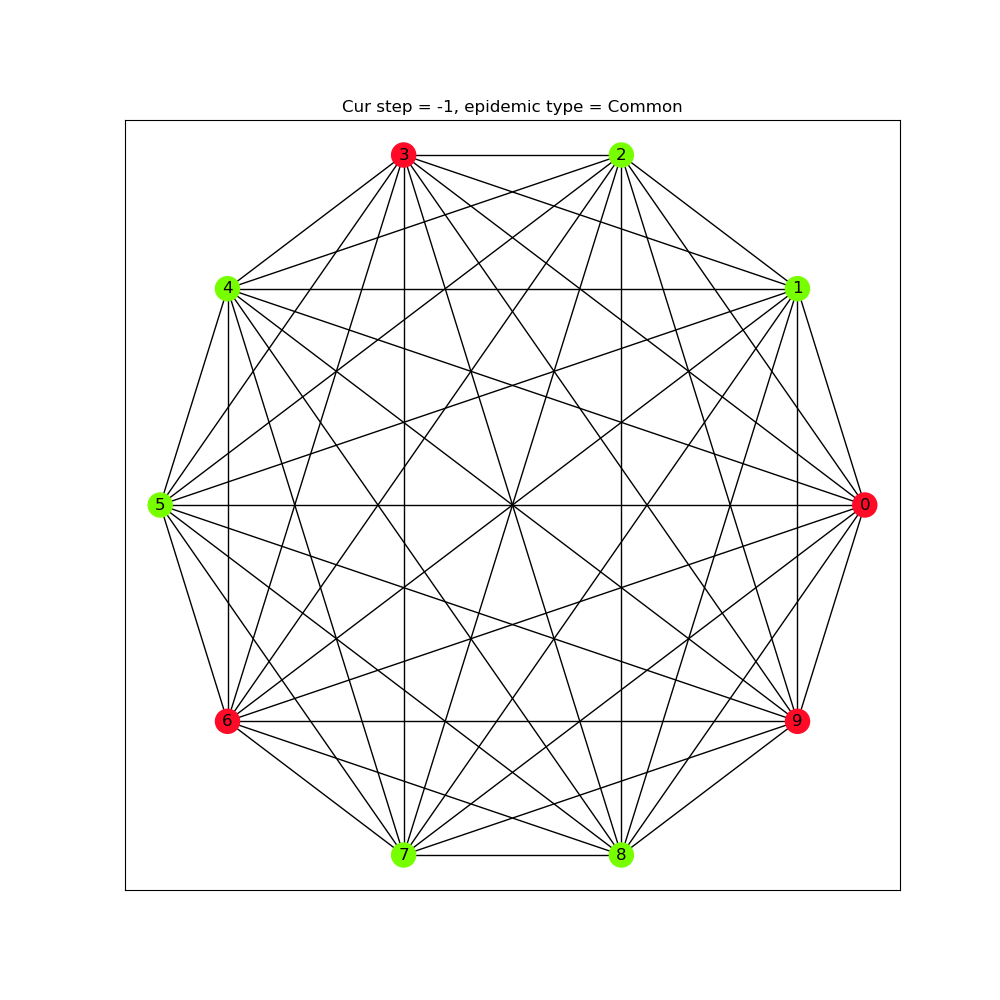
\includegraphics[width=0.32\linewidth, keepaspectratio]{../../figs/evidence2/init}}
				\subfigure[Введение карантина]{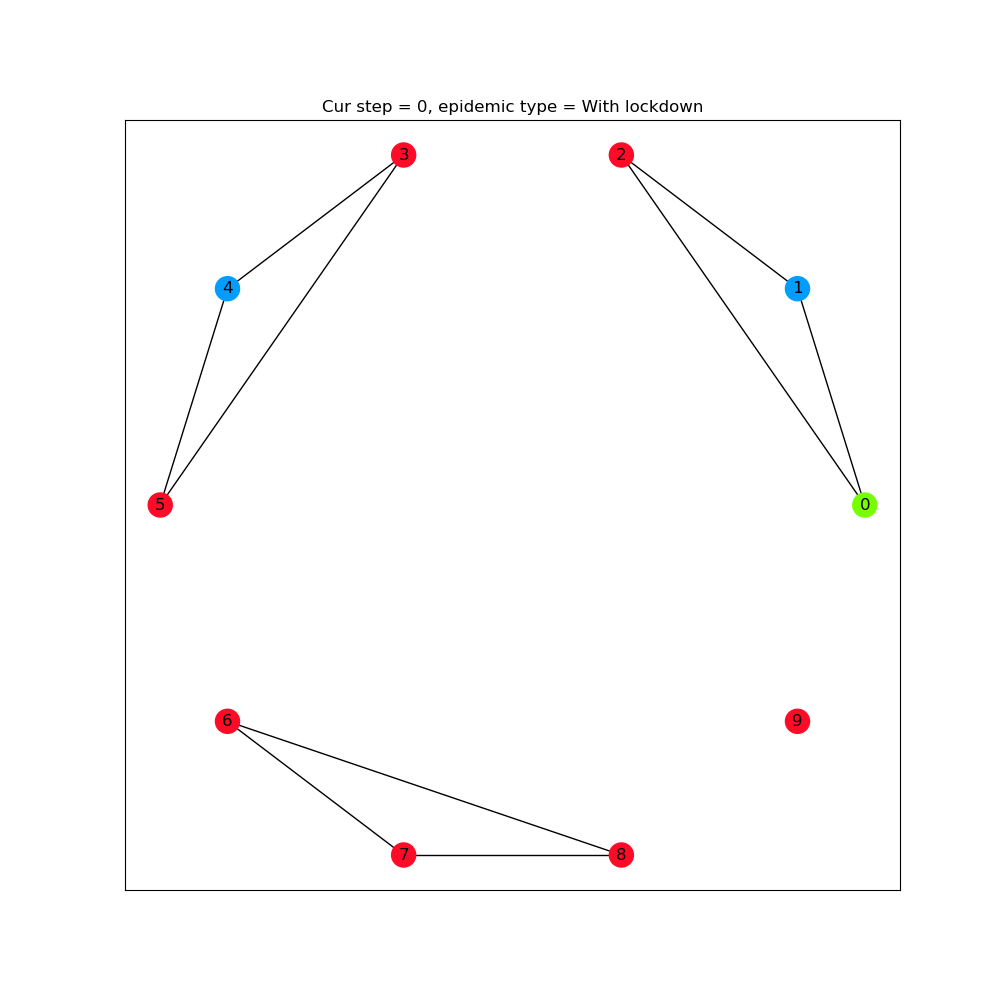
\includegraphics[width=0.32\linewidth, keepaspectratio]{../../figs/evidence2/start_with_ld.png}}
				\subfigure[Снятие карантина]{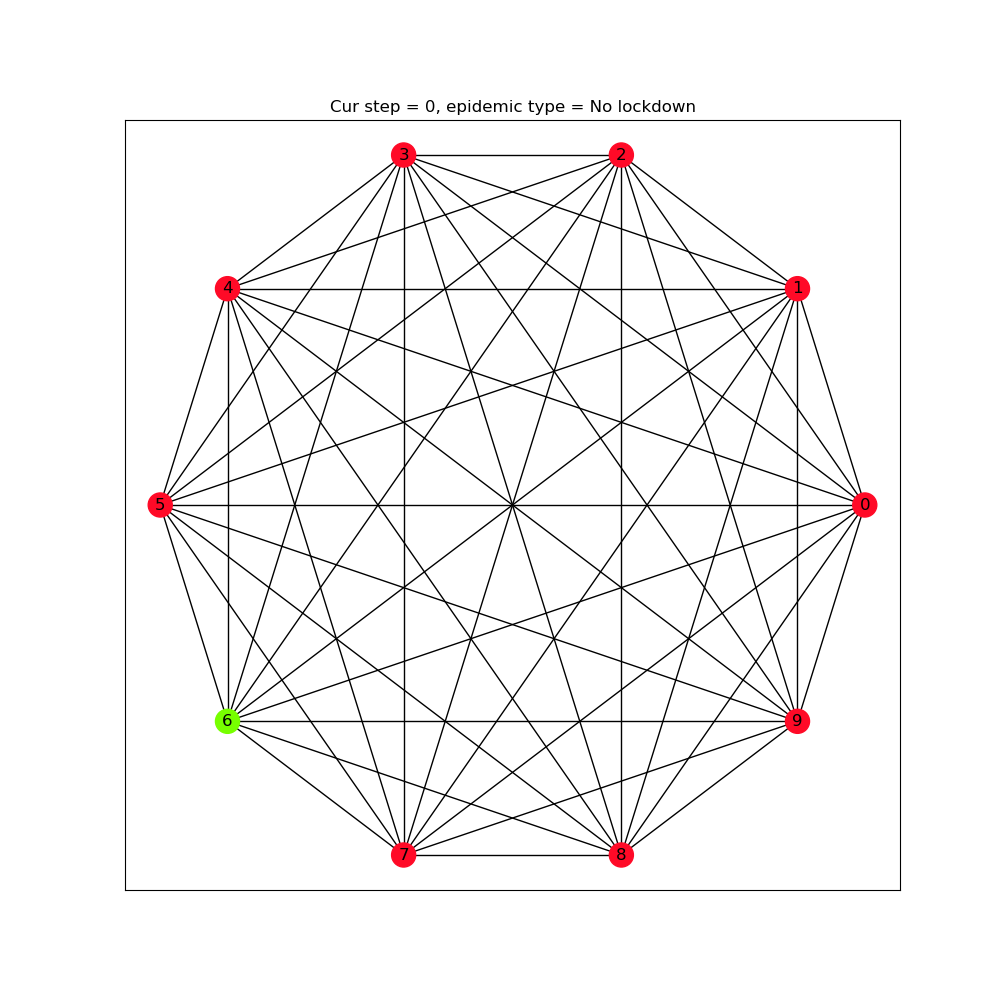
\includegraphics[width=0.32\linewidth, keepaspectratio]{../../figs/evidence2/start_no_ld.png}}
			\end{figure}
		
	\end{frame}

	\begin{frame}{Постановка задачи}
		
	Параметры эпидемии:
		
	\begin{itemize}
		\item $\gamma = \mathbb{P}(I \rightarrow R)$ --- вероятность "выздороветь"
		\item $\sigma = \mathbb{P}(R \rightarrow S)$ --- вероятность стать снова подверженным заболеванию.
		\item $\beta \sim \mathbb{P}(S \rightarrow I)$ --- "заразность" болезни.
	\end{itemize}
	
	$\mathbb{P}(S \rightarrow I)$ зависит от $\beta$ и от <<больных>> соседей данной вершины. Остальные переходы состояний вершин определяются только данными параметрами.  \medskip
	
	\textit{Задача}: выяснить, как ведут себя вероятности $ \mathbb{P}(S \in S / I / R) $ для всех вершин и как меняется их эволюция при введении локдауна?
		
	\end{frame}

	\begin{frame}{Теоретическая часть}
		Вероятность заразиться на след. шаге для здоровой вершины:
		\begin{equation*}
			\mathcal{P}(u \in I_{t+1} | u \in S_{t+1}) = 1 - \prod\limits_{v \in N(v)} (1 - \mathbb{P}(v \in I_t) \cdot \beta \cdot w_{uv})
		\end{equation*}
		
		Имеем $ 3^{|V|} $ состояний в цепи.
		
		\begin{figure}
			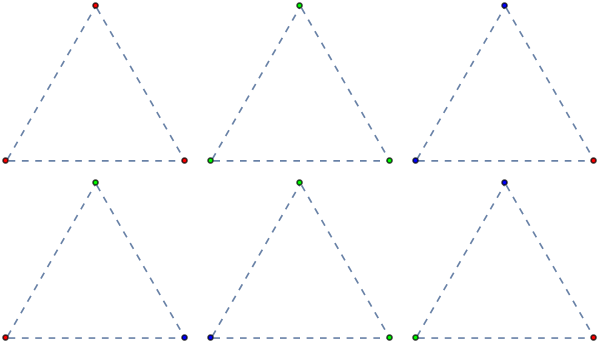
\includegraphics[width=0.5\linewidth, keepaspectratio]{img/states_in_chain}
			\caption{Часть множества состояний}
		\end{figure}		
	
	\end{frame}

	\begin{frame}{Теоретическая часть}
		В каждой вершине $ u $ живёт распределение $ (p_S^u, p_I^u, p_R^u)^T $, с которым удобно работать. Уравнения на их динамику:
		
		\begin{align*}
			\mathbb{P}(v \in S_{t+1}) &= \gamma \mathbb{P}(v \in R_t) + \mathbb{P}(v \in S_t) \cdot \underbrace{\prod\limits_{u \in N(v)} (1 - \mathbb{P}(u \in I_t) \beta w_{uv})}_{A_v} \\
			\mathbb{P}(v \in I_{t+1}) &= (1 - \sigma) \mathbb{P}(v \in I_t) + \mathbb{P}(v \in S_t) \cdot (1 - A_v) \\
			\mathbb{P}(v \in R_{t+1}) &= \sigma \mathbb{P}(v \in I_t) + (1 - \gamma) \mathbb{P}(v \in R_t) 
		\end{align*}
				
		
	\end{frame}

	\begin{frame}{Теоретическая часть}
		Аналогично можно написать и для матожиданий:
		
		\begin{align*}
			\matwait(\#S_{t+1}) &= \gamma \matwait(\#R_{t}) + \sum\limits_{v \in V} \prob(v \in S_t) A_v \\
			\matwait(\#I_{t+1}) &= (1 - \sigma) \matwait(\#I_{t}) + \matwait(\#S_{t}) - \sum\limits_{v \in V} \prob(v \in S_t) A_v \\
			\matwait(\#R_{t+1}) &=  \sigma \matwait(\# I_t) + (1 - \gamma) \matwait(\#R_{t})
		\end{align*}
		
		Отсюда следует простое \textit{условие на локальное увеличения ожидаемого числа больных}:
		
		\begin{equation*}
			\matwait(\#I_{t}) \le \frac{1}{\sigma} \matwait(\#S_{t}) \Rightarrow \matwait(\#I_{t+1}) \ge \matwait(\#I_{t})
		\end{equation*}
		
	\end{frame}

	\begin{frame}{Теоретическая часть}
	 Из нелинейной системы получим линейную:
	 
	 	\[ A_v = \prod\limits_{u \in N(v)} (1 - \mathbb{P}(u \in I_t) \beta w_{uv}) \]
		
		\begin{equation*}
			\begin{cases}
				\prob(v \in S_{t+1}) &= \gamma (1 - \prob(u \in I_t) - \prob(u \in S_t)) + \prob(v \in S_t) \cdot A_v \\
				\prob(v \in I_{t+1}) &= (1 - \sigma) \prob(v \in I_t) + \prob(v \in S_t) \cdot (1 - A_v)
			\end{cases}
		\end{equation*}
	\centering $ \Downarrow $
		\begin{equation*}
			\begin{cases}
				\prob(v \in S_{t+1}) &\le \gamma (1 - \prob(u \in I_t) - \prob(u \in S_t)) + (1 - \beta \sum\limits_{u \in N(v)} w_{uv} \prob(u \in I_t)) \\
				\prob(v \in I_{t+1}) &\le (1 - \sigma) \prob(v \in I_t) + \prob(v \in S_t) \cdot \beta \sum\limits_{u \in N(v)} w_{uv} \prob(u \in I_t) 
			\end{cases}
		\end{equation*}
			\end{frame}

	\begin{frame}{Теоретическая часть}
		Работаем только с этой рекуррентой:
		
		\begin{equation*}
			\prob(v \in I_{t+1}) = (1 - \sigma) \prob(v \in I_t) + \beta \sum\limits_{u \in N(v)} w_{uv} \prob(u \in I_t)
		\end{equation*}
	
	Ищем решение в виде: $ \mathbf{P} = \mathbf{e} \cdot q^n$, где $\mathbf{e}$ --- некоторый вектор. В итоге всё сведётся к решению СЛАУ:
	
	\begin{gather*}
		e_k q^{n+1} = (1 - \sigma) e_k q^n \sum\limits_{j \not= k} \beta \omega_{jk} e_j q^n \\
		\sum\limits_{j \not= k} \omega_{jk} e_j - \frac{q + \sigma - 1}{\beta} e_k = 0, \  \forall k \in \overrightarrow{1, |V|}
	\end{gather*}
		
	\end{frame}

	\begin{frame}{Эксперимент}
		\renewcommand{\thesubfigure}{}
		
		\begin{figure}
			\subfigure[Стандартный граф]{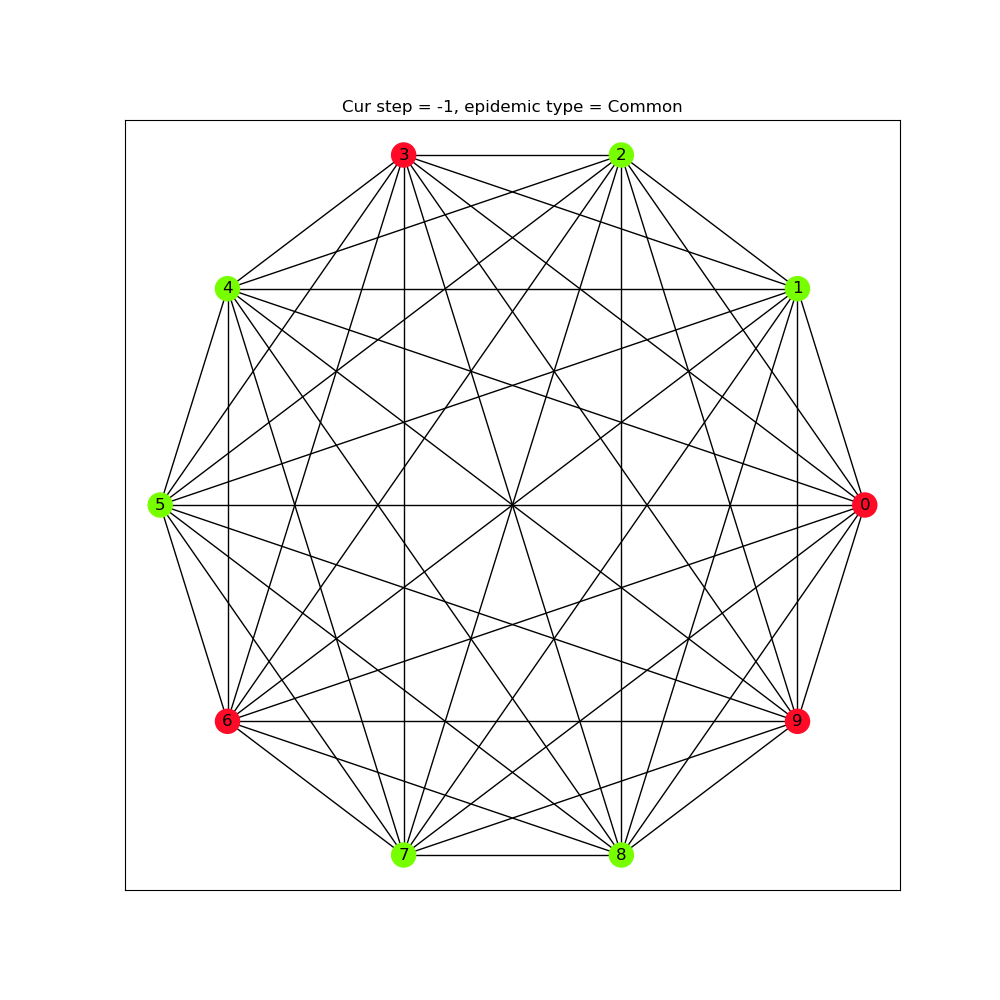
\includegraphics[width=0.49\linewidth, keepaspectratio]{../../figs/evidence2/init}}
			\subfigure[Граф локдауна]{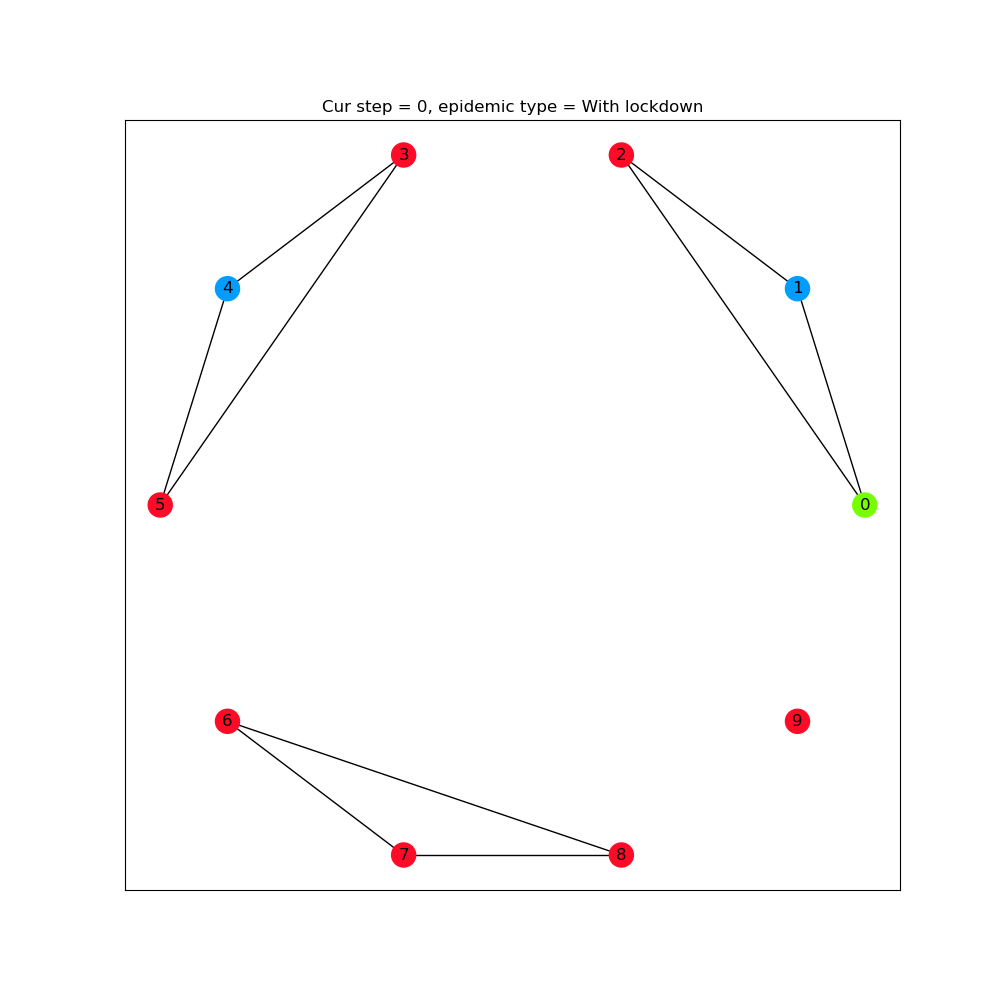
\includegraphics[width=0.49\linewidth, keepaspectratio]{../../figs/evidence2/start_with_ld}}
		\end{figure}

	\begin{center}
		\textbf{{\large Полный граф}}
	\end{center}
		
	\end{frame}

	\begin{frame}{Эксперимент}
		\renewcommand{\thesubfigure}{}
		
		\begin{figure}
			\subfigure[Стандартный граф]{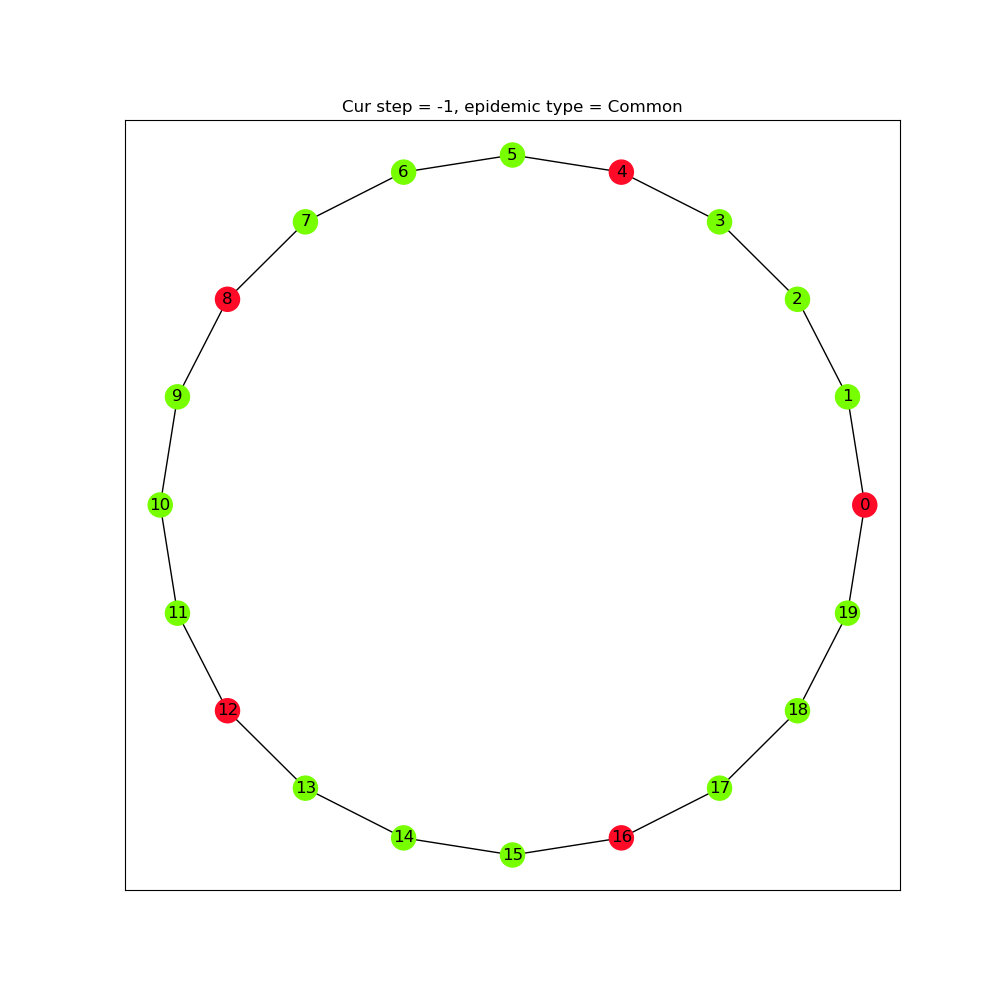
\includegraphics[width=0.49\linewidth, keepaspectratio]{../../figs/evidence3/init}}
			\subfigure[Граф локдауна]{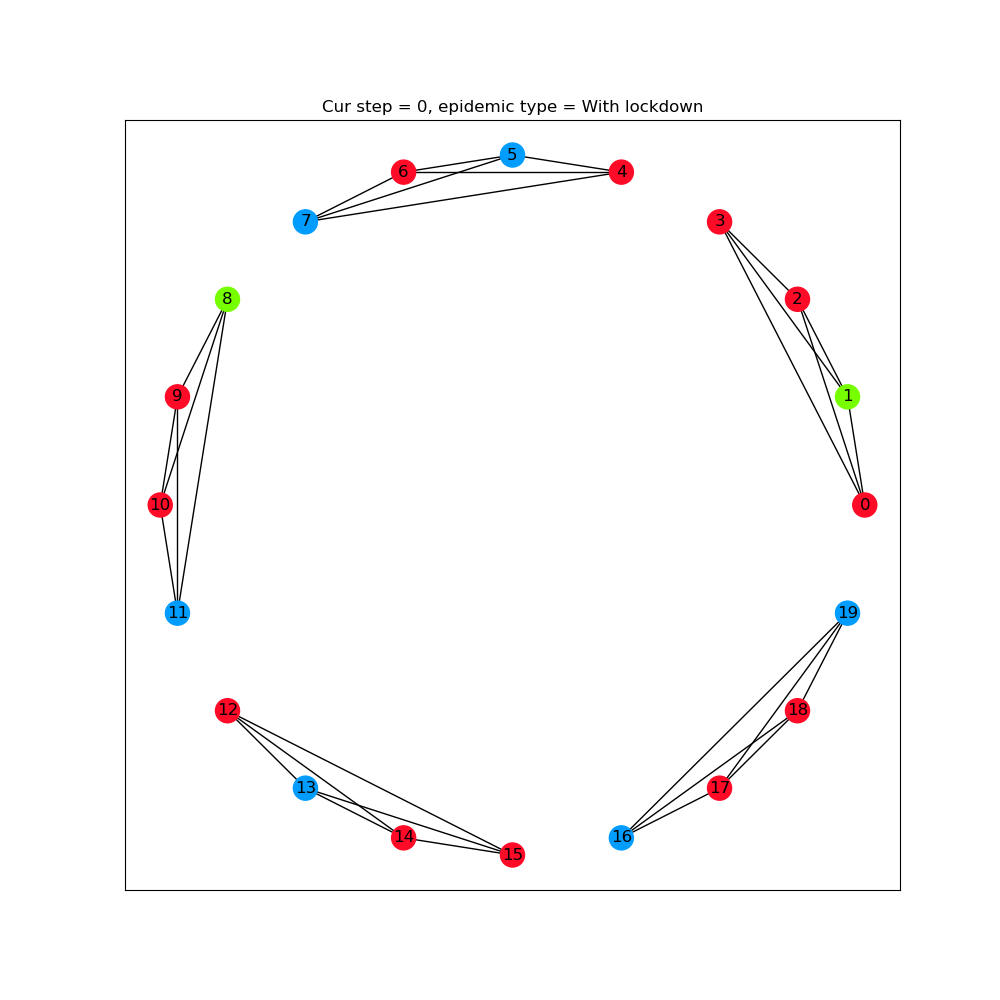
\includegraphics[width=0.49\linewidth, keepaspectratio]{../../figs/evidence3/start_with_ld}}
		\end{figure}
	
	\begin{center}
		\textbf{{\large Граф-цикл}}
	\end{center}
		
	\end{frame}

	\begin{frame}{Эксперимент}
		\begin{figure}
			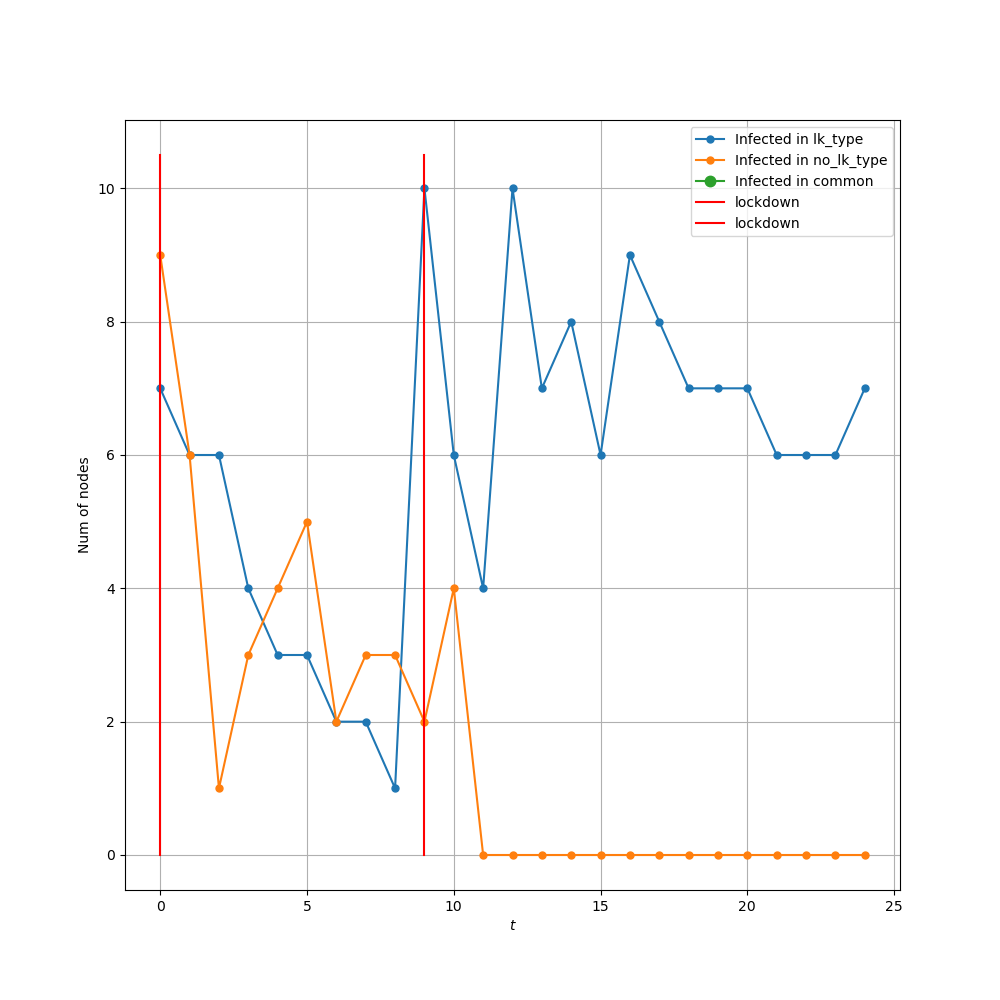
\includegraphics[width=0.49\linewidth, keepaspectratio]{../../figs/evidence2/tracks.png}
			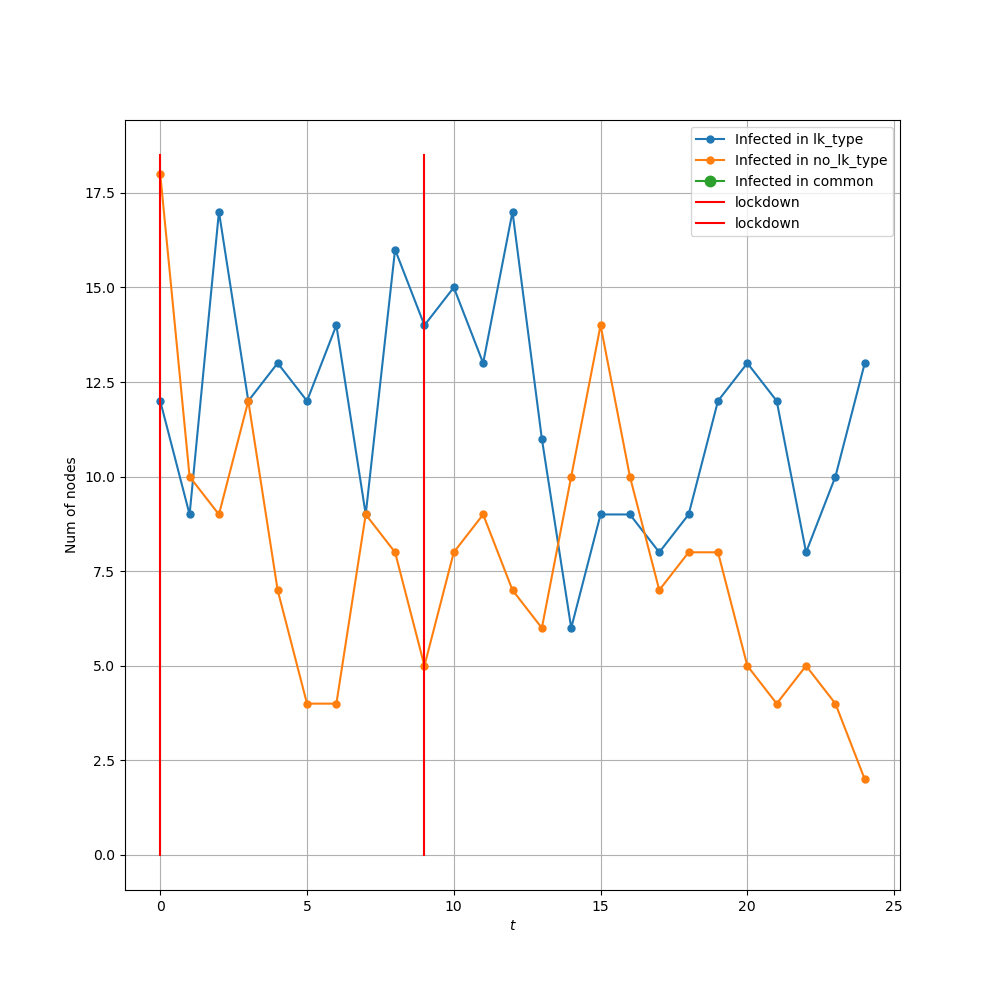
\includegraphics[width=0.49\linewidth, keepaspectratio]{../../figs/evidence3/tracks.png}
			\caption{Треки изменения кол-ва вершин в разных состояниях}
		\end{figure}
	\end{frame}

	\begin{frame}{Эксперимент}
		\begin{figure}
			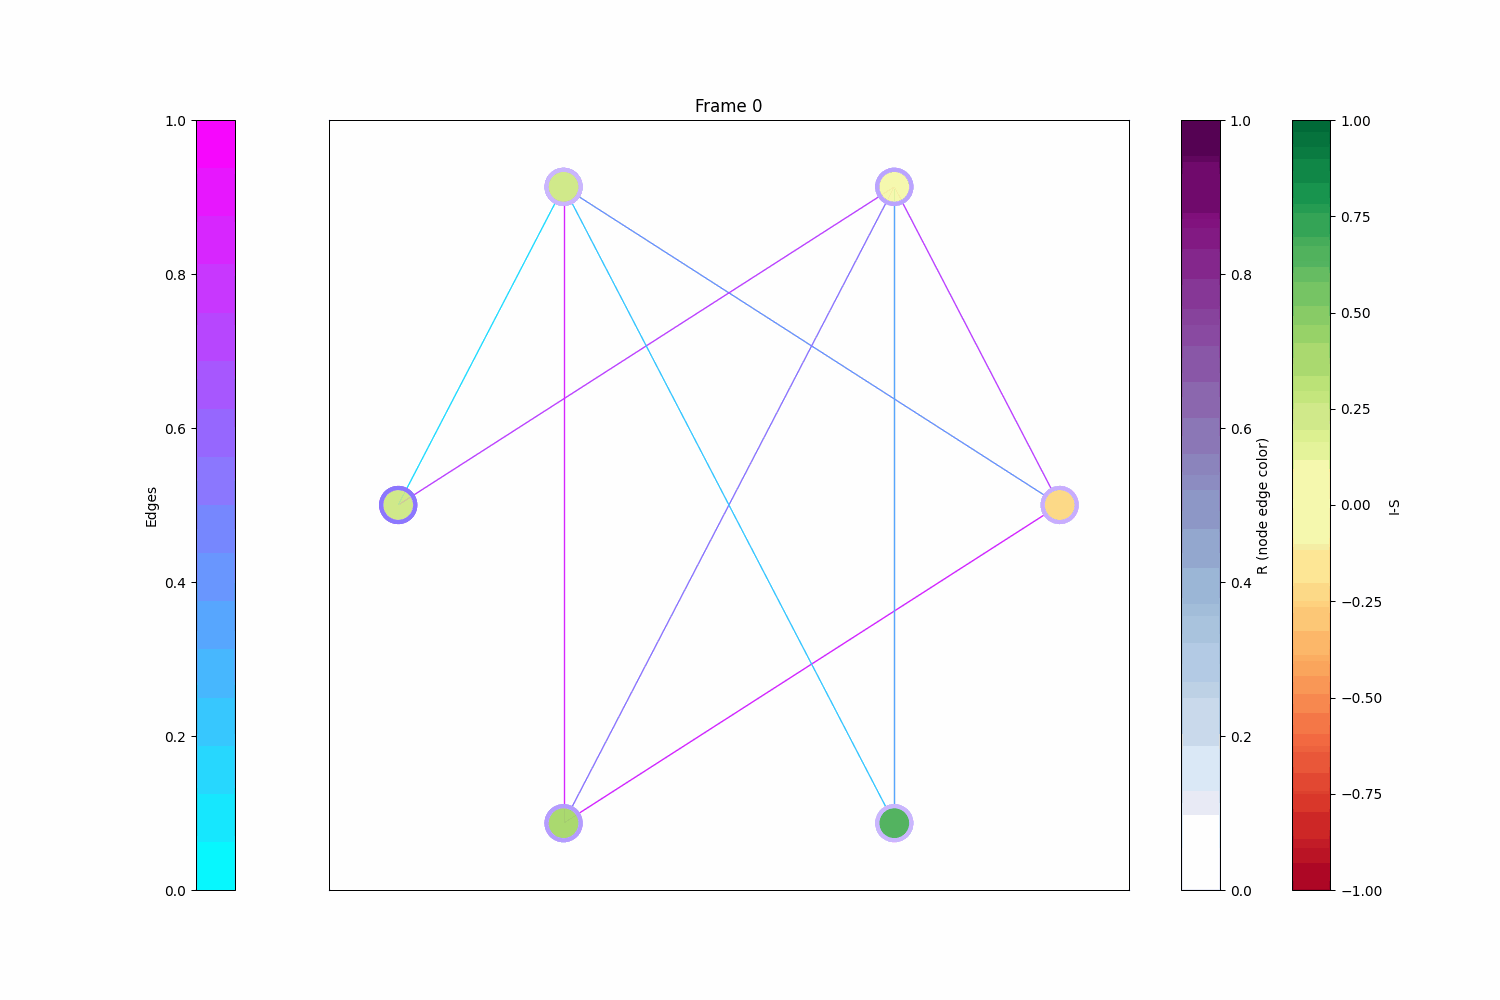
\includegraphics[width=\linewidth, keepaspectratio]{./img/0.png}
			\caption{Эволюция вероятностей в цепи Маркова}
		\end{figure}
	\end{frame}

		\begin{frame}{Эксперимент}
		\begin{figure}
			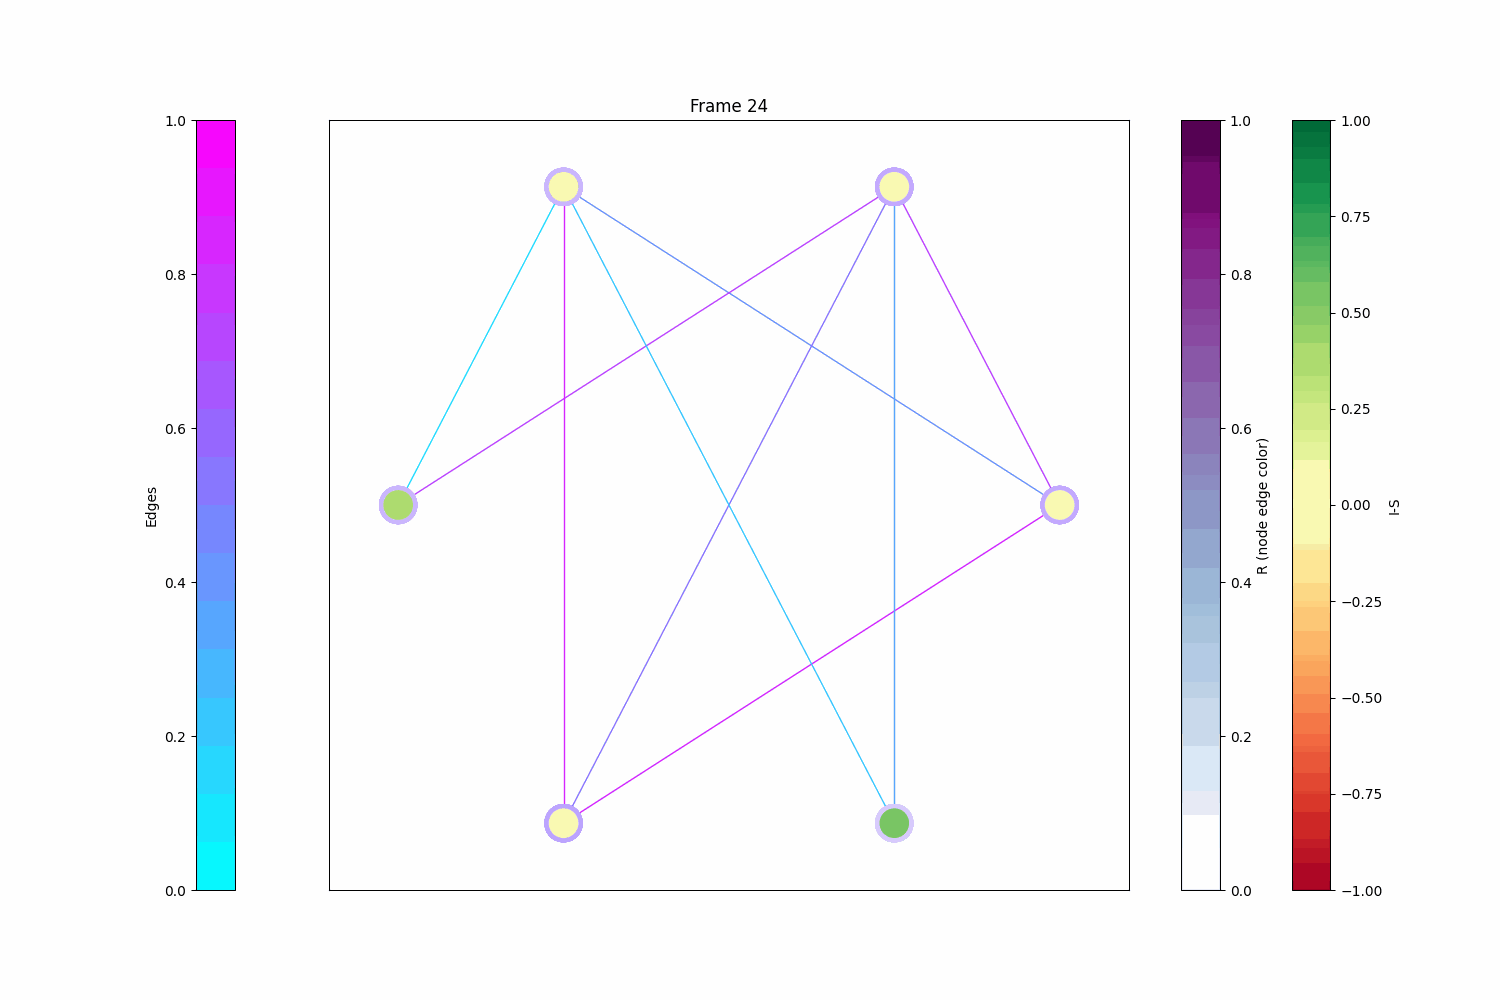
\includegraphics[width=\linewidth, keepaspectratio]{./img/24.png}
			\caption{Эволюция вероятностей в цепи Маркова}
		\end{figure}
	\end{frame}

	\begin{frame}{Заключение}
		\begin{itemize}
			\item Задача распространения эпидемий формализована в виде марковских цепей
			\item Для любого графа и любого начального распределения больных, после достаточно большого времени эпидемия затухнет
			\item Возможно получить точные уравнения и оценки на скорость этого затухания
			\item Негативное влияние локдауна подтверждено эмпирически 
		\end{itemize}
	\end{frame}
	
\end{document}